\documentclass[11pt]{article}
\usepackage[english]{babel}
\usepackage[left=1in,right=1in,top=1in,bottom=0.9in]{geometry}
\usepackage{graphicx}
\graphicspath{{figures/}}
\usepackage{amsmath}
\usepackage{amssymb}
\usepackage{booktabs}
\usepackage{setspace}
\usepackage[authoryear,round]{natbib}
\usepackage{hyperref}
\hypersetup{colorlinks=true, linkcolor=black, citecolor=black, urlcolor=black}

\title{\vspace{-4em}\textbf{Confidence-Weighted Pair Trading via DCC-eGARCH}
\thanks{Code and replication data are available at \href{https://github.com/Softpandaa/confidence-pair-trading}{\textit{GitHub}}.}}
\author{Samson LAM \qquad Angus CHEUNG \qquad Benny NG \qquad Edward SIN}
\date{April 2024}

\newcommand{\EWFE}{\mbox{EW-FE}}
\newcommand{\EWOE}{\mbox{EW-OE}}
\newcommand{\OWOE}{\mbox{OW-OE}}

\begin{document}
\maketitle
\vspace{-2em}

\section{Introduction}

A pair trade holds offsetting positions in two assets whose prices share a long-run equilibrium, and profits when a temporary deviation from that equilibrium closes. Three design choices govern such a strategy. The first is which pairs to trade, the second is when to enter and exit, and the third is how much capital each pair receives. This project holds the first fixed and tests the second and third against each other.

We backtest cointegration-based pair trading strategies from a pool of US equities and ETFs, over an evaluation window running from August 2021 to December 2023. Hedge ratios are time-varying and estimated by the Kalman filter of \citet{kalman1960}. Spread volatility is modeled by the exponential GARCH of \citet{nelson1991} within the dynamic conditional correlation framework of \citet{engle2002}. We optimize the entry and exit thresholds, and propose a confidence-weighting scheme based on the rolling cointegration statistic and forecast volatility. We found that optimizing the thresholds alone hurt risk-adjusted return, but together with the confidence weighting reverses that and delivers the highest return, the highest Sharpe ratio and the lowest drawdown.

Section 2 describes the data and forms the pairs. Section 3 models the spread volatility. Section 4 defines and optimizes the trading signal. Section 5 sets out the weighting scheme. Section 6 reports the backtest and Section 7 concludes.

\section{Pair Formation}

\subsection{Data}

The asset pool is 45 US equities and ETFs of large market capitalization and high liquidity, listed in Table \ref{tab:pool}. It spans commodities, technology, healthcare, banking, energy, consumer staples and real estate. Daily closing prices are taken from January 2012 to December 2023, and names without a complete price history over that period are excluded. We apply an 80-20 train-test split, so the training set covers January 2012 to 5 August 2021 and the testing set covers 6 August 2021 to December 2023.

\begin{table}[thbp]
\centering
\begin{tabular}{llllll}
\toprule
GDX  & GDXJ  & GLD  & AAPL & GOOGL & AMD  \\
NVDA & CSCO  & ORCL & TTWO & EA    & HYG  \\
LQD  & JNK   & SLV  & USLV & SIVR  & USO  \\
QQQ  & SPY   & VOO  & VDE  & VTI   & VDC  \\
KXI  & IBB   & VHT  & VNQ  & IYR   & MSFT \\
PG   & TMF   & UPRO & WFC  & JPM   & GS   \\
CVX  & XOM   & INTC & COST & WMT   & T    \\
VZ   & CMCSA & AMZN &      &       &      \\
\bottomrule
\end{tabular}
\caption{Asset pool screened for pairs formation.}
\label{tab:pool}
\end{table}

\subsection{Cointegration}

Two price series $x_t$ and $y_t$ are cointegrated when the spread
\begin{equation}
s_t = y_t - (\beta_t x_t + \alpha_t)
\label{eq:spread}
\end{equation}
is (weakly) stationary. We test stationarity using the two-step procedure of \citet{engle1987}, and retain a pair when the null of no cointegration is rejected at the 5\% level. Figure \ref{fig:heatmap} shows the resulting p-values over all $\binom{45}{2}$ candidates. 73 pairs are significant and are carried forward, spanning 38 distinct tickers.

\begin{figure}[thbp]
\centering
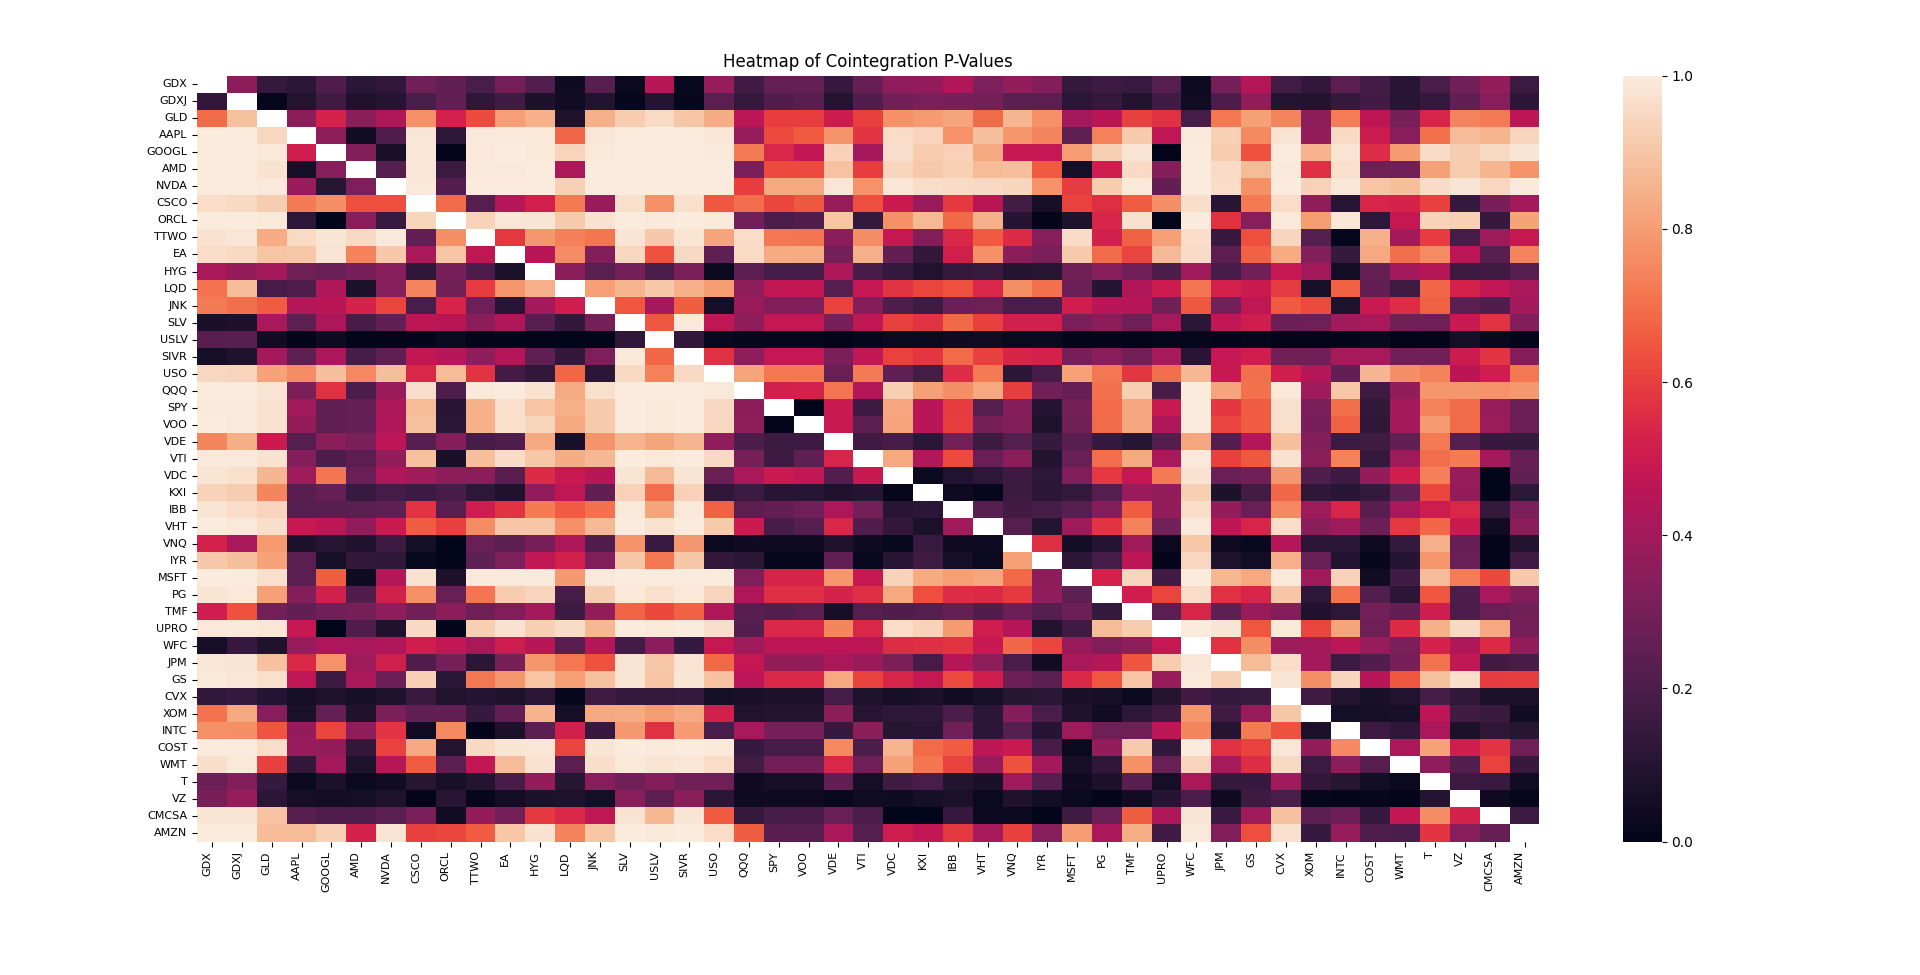
\includegraphics[width=0.92\textwidth]{Heatmap of Cointegrated Pair P-Values.png}
\caption{Engle-Granger p-values for every candidate pair on the training sample. Darker cells indicate stronger evidence of cointegration.}
\label{fig:heatmap}
\end{figure}

\subsection{Time-varying Hedge Ratio}

Market conditions and relative volatility move over time, so a hedge ratio estimated once by least squares will drift out of date. We therefore treat $(\alpha_t, \beta_t)$ in equation \eqref{eq:spread} as a latent state following a random walk, and estimate it with the Kalman filter of \citet{kalman1960}. Writing the state as $\boldsymbol{\phi}_t = (\alpha_t, \beta_t)^\top$,
\begin{equation}
\begin{aligned}
\boldsymbol{\phi}_t &= \boldsymbol{\phi}_{t-1} + \omega_t, \qquad \omega_t \sim N(0, \delta I), \\
y_t &= (1, x_t)\, \boldsymbol{\phi}_t + \nu_t, \qquad \nu_t \sim N(0, \sigma_\nu^2),
\end{aligned}
\end{equation}
with the state noise scale set to $\delta = 10^{-3}$ and the observation variance to $\sigma_\nu^2 = 2$. We pass each price series through a univariate Kalman smoother before running the regression to remove transient noise. Then, we evaluate the spread in equation \eqref{eq:spread} at the filtered state.

\subsection{Half Life}

The rolling window used later to compute the mean, volatility and z-score of each spread is set by the speed at which that spread reverts. Regressing the spread increment on its lagged level,
\begin{equation}
\Delta s_t = \kappa\, s_{t-1} + \epsilon_t, \qquad H = -\frac{\ln 2}{\kappa},
\end{equation}
gives the half-life $H$, the number of days over which a deviation is expected to halve. Each pair uses its own $H$, rounded to whole days, as its window length.

\section{Volatility Clustering}

We test the spread for normality with the SW test of \citet{shapiro1965}, which measures departure from normality, and the JB test of \citet{jarque1980}, which compares skewness and kurtosis to the Gaussian case. In the training sample, no pair is consistent with normality at the 5\% level under either test, and Q-Q plots in the Appendix show heavier tails than the Gaussian. We therefore adopt a Student t conditional distribution throughout.

\subsection{Exponential GARCH}

\citet{engle1982} introduced the autoregressive conditional heteroskedasticity model (ARCH), which has since been extended in several directions. The exponential form of \citet{nelson1991} is used here for two reasons. It admits an asymmetric response, so that a negative shock at $t-1$ raises the variance at $t$ by more than a positive shock of the same size, which is the leverage effect. It also models the logarithm of the variance, so that positivity holds for any parameter values. 
\begin{equation}
\begin{aligned}
\varepsilon_t &= h_t \eta_t, \qquad \eta_t \sim \text{Student t}(0,1) \\
\ln h_t^2 &= \omega_h + \sum_{i=1}^{p} \Big( a_i \big| \eta_{t-i} - \mathbb{E}|\eta_{t-i}| \big| + \lambda_i \eta_{t-i} \Big) + \sum_{j=1}^{q} b_j \ln h_{t-j}^2
\end{aligned}
\end{equation}
where $h_t$ is the conditional volatility, $\omega_h$ the constant, $a_i$ the ARCH coefficients, $b_j$ the GARCH coefficients and $\lambda_i$ the leverage coefficients.

The choices of $p$ and $q$ are screened over the set $\{1,2,3,4,5\}$, evaluated by the Akaike and Bayesian information criteria, whose mean and median across pairs are shown in Figure \ref{fig:ic}. The Bayesian criterion is minimized at $p = 3$ and $q = 1$ on both the mean and the median, and Akaike draws a similar conclusion.

\begin{figure}[thbp]
\centering
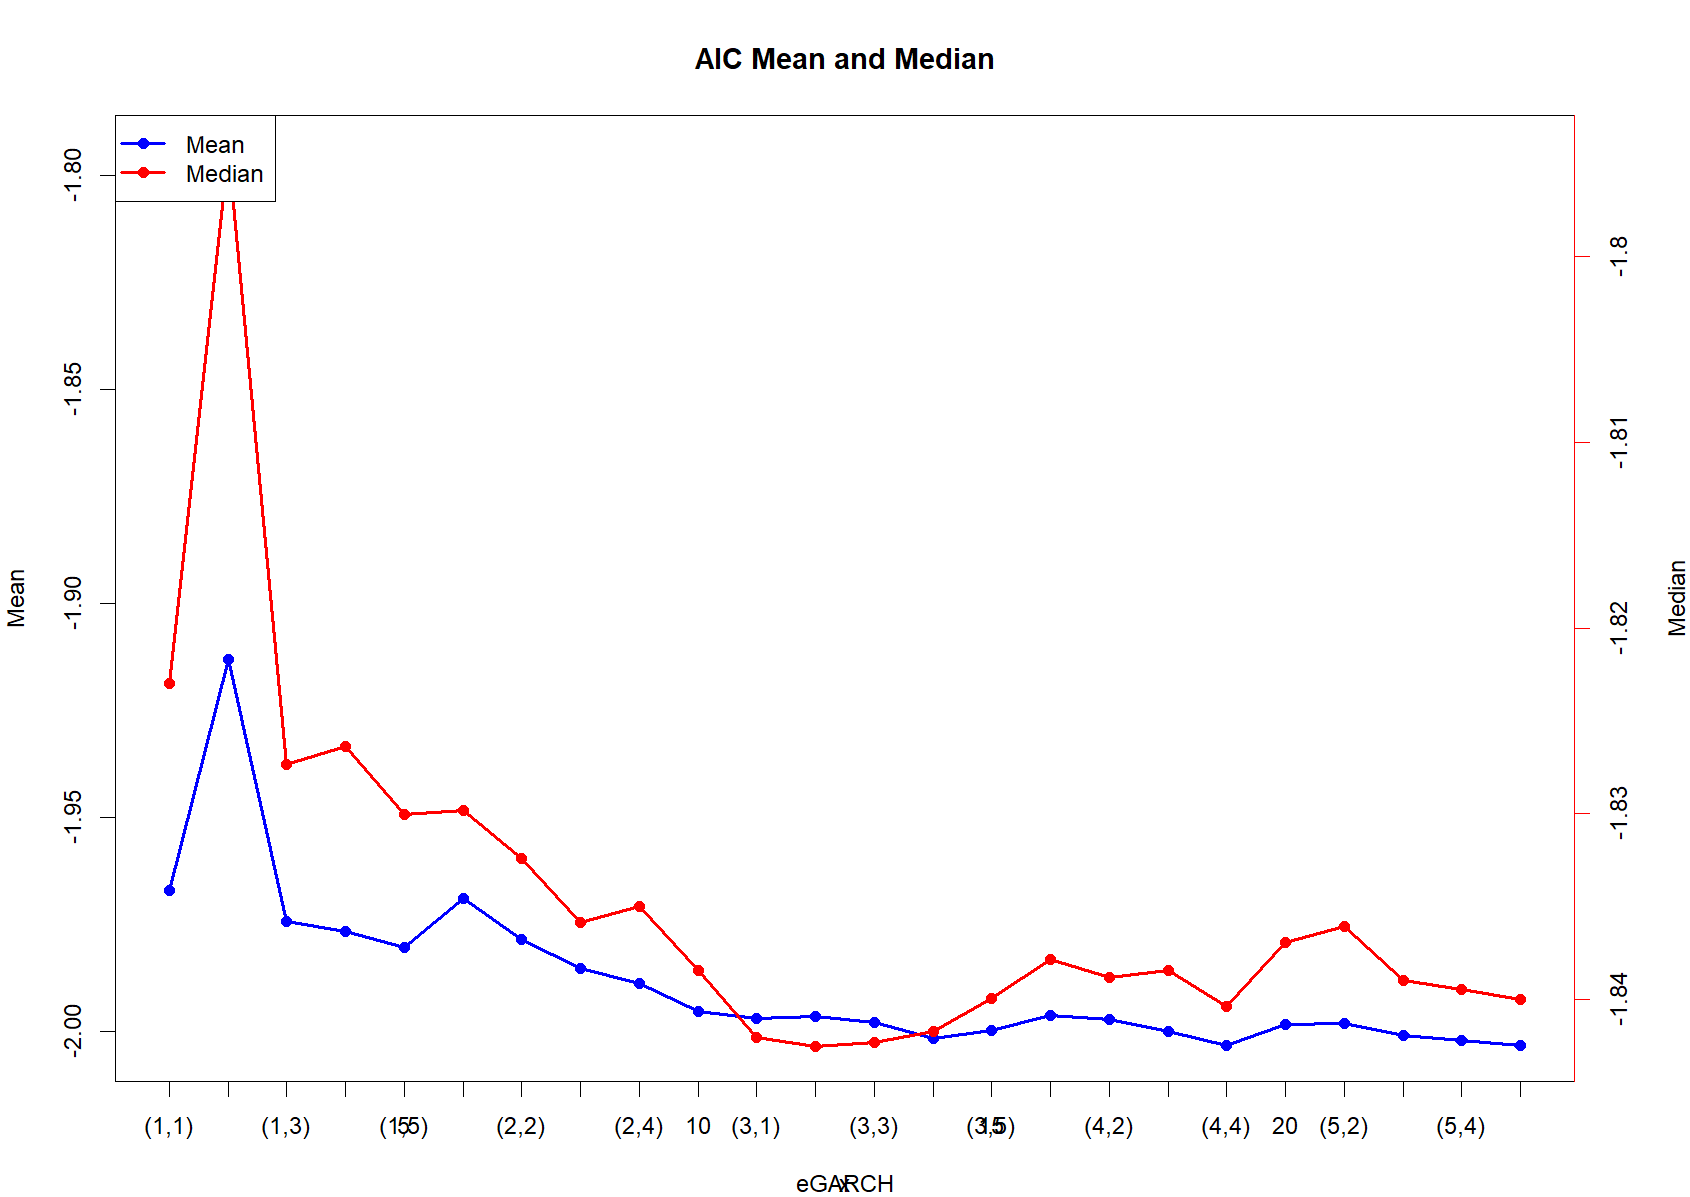
\includegraphics[width=0.45\textwidth]{AIC_mean_median.jpeg}
\hfill
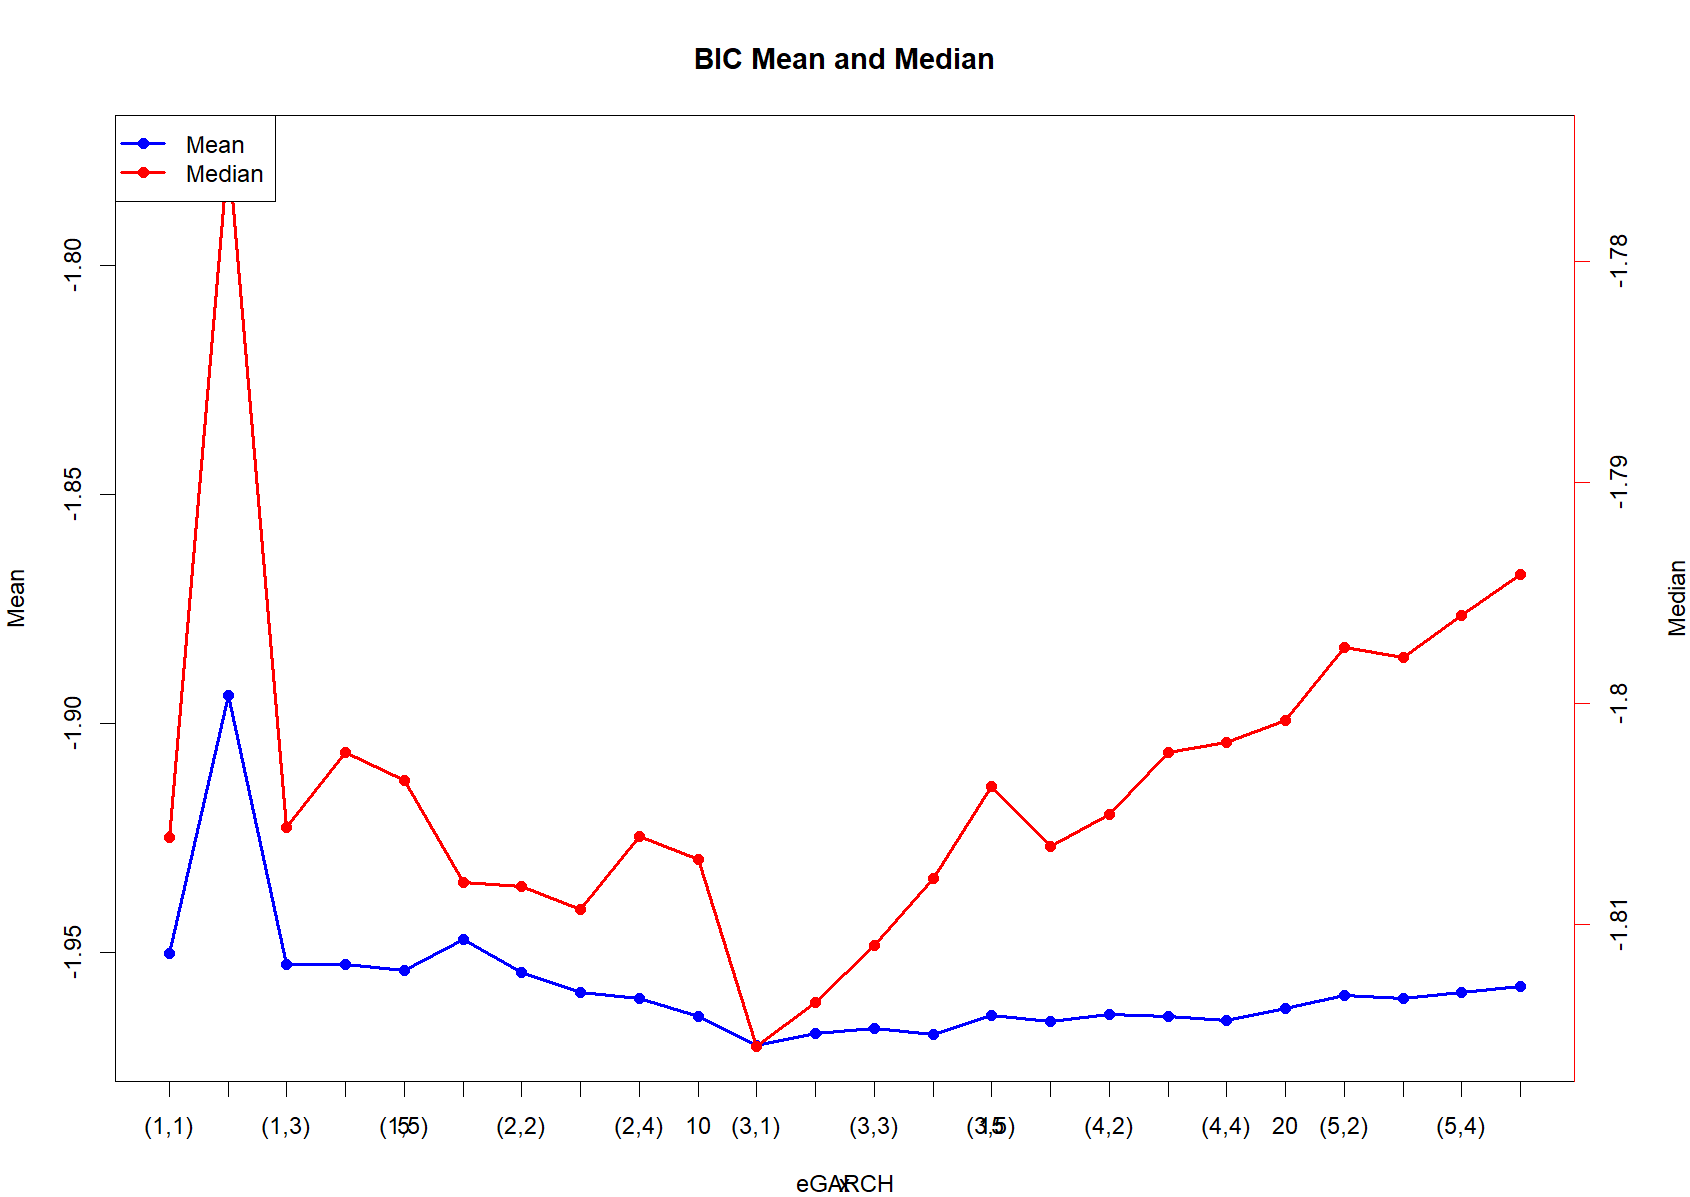
\includegraphics[width=0.45\textwidth]{BIC_mean_median.jpeg}
\caption{Akaike and Bayesian information criterion by eGARCH order.}
\label{fig:ic}
\end{figure}

\subsection{Dynamic Conditional Correlation}

The 73 spreads are not independent, so we estimate their volatilities jointly under the dynamic conditional correlation model of \citet{engle2002}. Let $s_t$ denote the spreads at time $t$ and $\mu$ their conditional means. Standardizing by the diagonal matrix of conditional volatilities gives
\begin{equation}
v_t = D_t^{-1}(s_t - \mu), \qquad D_t = \mathrm{diag}(h_{1t}, h_{2t}, \ldots, h_{mt}),
\end{equation}
and the quasi-correlation matrix evolves as
\begin{equation}
Q_t = (1 - \theta_1 - \theta_2)\bar{Q} + \theta_1 v_{t-1} v_{t-1}^\top + \theta_2 Q_{t-1},
\label{eq:dcc}
\end{equation}
where $\theta_1$ and $\theta_2$ govern the persistence of the process and $\bar{Q}$ is its unconditional level. Denoting by $T_0 = \lceil T/3 \rceil$ the end of the burn-in period, which is discarded so that the starting value does not contaminate the average,
\begin{equation}
\bar{Q} = \frac{1}{T - T_0 + 1} \sum_{t = T_0}^{T} v_{t-1} v_{t-1}^\top .
\end{equation}

Fitted on the training spreads with multivariate Student t innovations, the persistence parameters are $\hat{\theta}_1 = 0.123$ and $\hat{\theta}_2 = 0.672$. Over the testing sample, equation \eqref{eq:dcc} is iterated forward and the conditional volatility of each spread is extracted for the trading signal at every date.

\section{Trading Signal}

\subsection{Definition}

Each spread is standardized with $\mu_{i,t}$ the rolling mean of spread $i$ over its half life window and $h_{i,t}$ is the conditional volatility,
\begin{equation}
z_{i,t} = \frac{s_{i,t} - \mu_{i,t}}{h_{i,t}},
\end{equation}
A position is opened when the z-score crosses an entry threshold and closed when it crosses the corresponding exit threshold, so that four parameters describe the rule. These are the long entry threshold LET, the long exit threshold LETX, the short entry threshold SET and the short exit threshold SETX. Crossings are strict, in the sense that the threshold must lie between consecutive observations,
\begin{align*}
\text{long entry} \quad & z_{i,t} < \text{LET}_i < z_{i,t-1}, &
\text{long exit} \quad & z_{i,t-1} < \text{LETX}_i < z_{i,t}, \\
\text{short entry} \quad & z_{i,t-1} < \text{SET}_i < z_{i,t}, &
\text{short exit} \quad & z_{i,t} < \text{SETX}_i < z_{i,t-1}.
\end{align*}

\subsection{Threshold Optimization}

Two objectives are considered: profit and Sharpe ratio. In both cases, the four thresholds are optimized by the Nelder-Mead simplex separately for each pair. Figure \ref{fig:zoptim} reports the distribution of the fitted thresholds and Figure \ref{fig:zdesc} reports their summary statistics under both objectives. The long entry threshold concentrates between $-0.70$ and $-0.65$, the long exit threshold near $0.05$, the short entry threshold between $0.60$ and $0.65$ and the short exit threshold near $-0.05$. 

\begin{figure}[thbp]
\centering
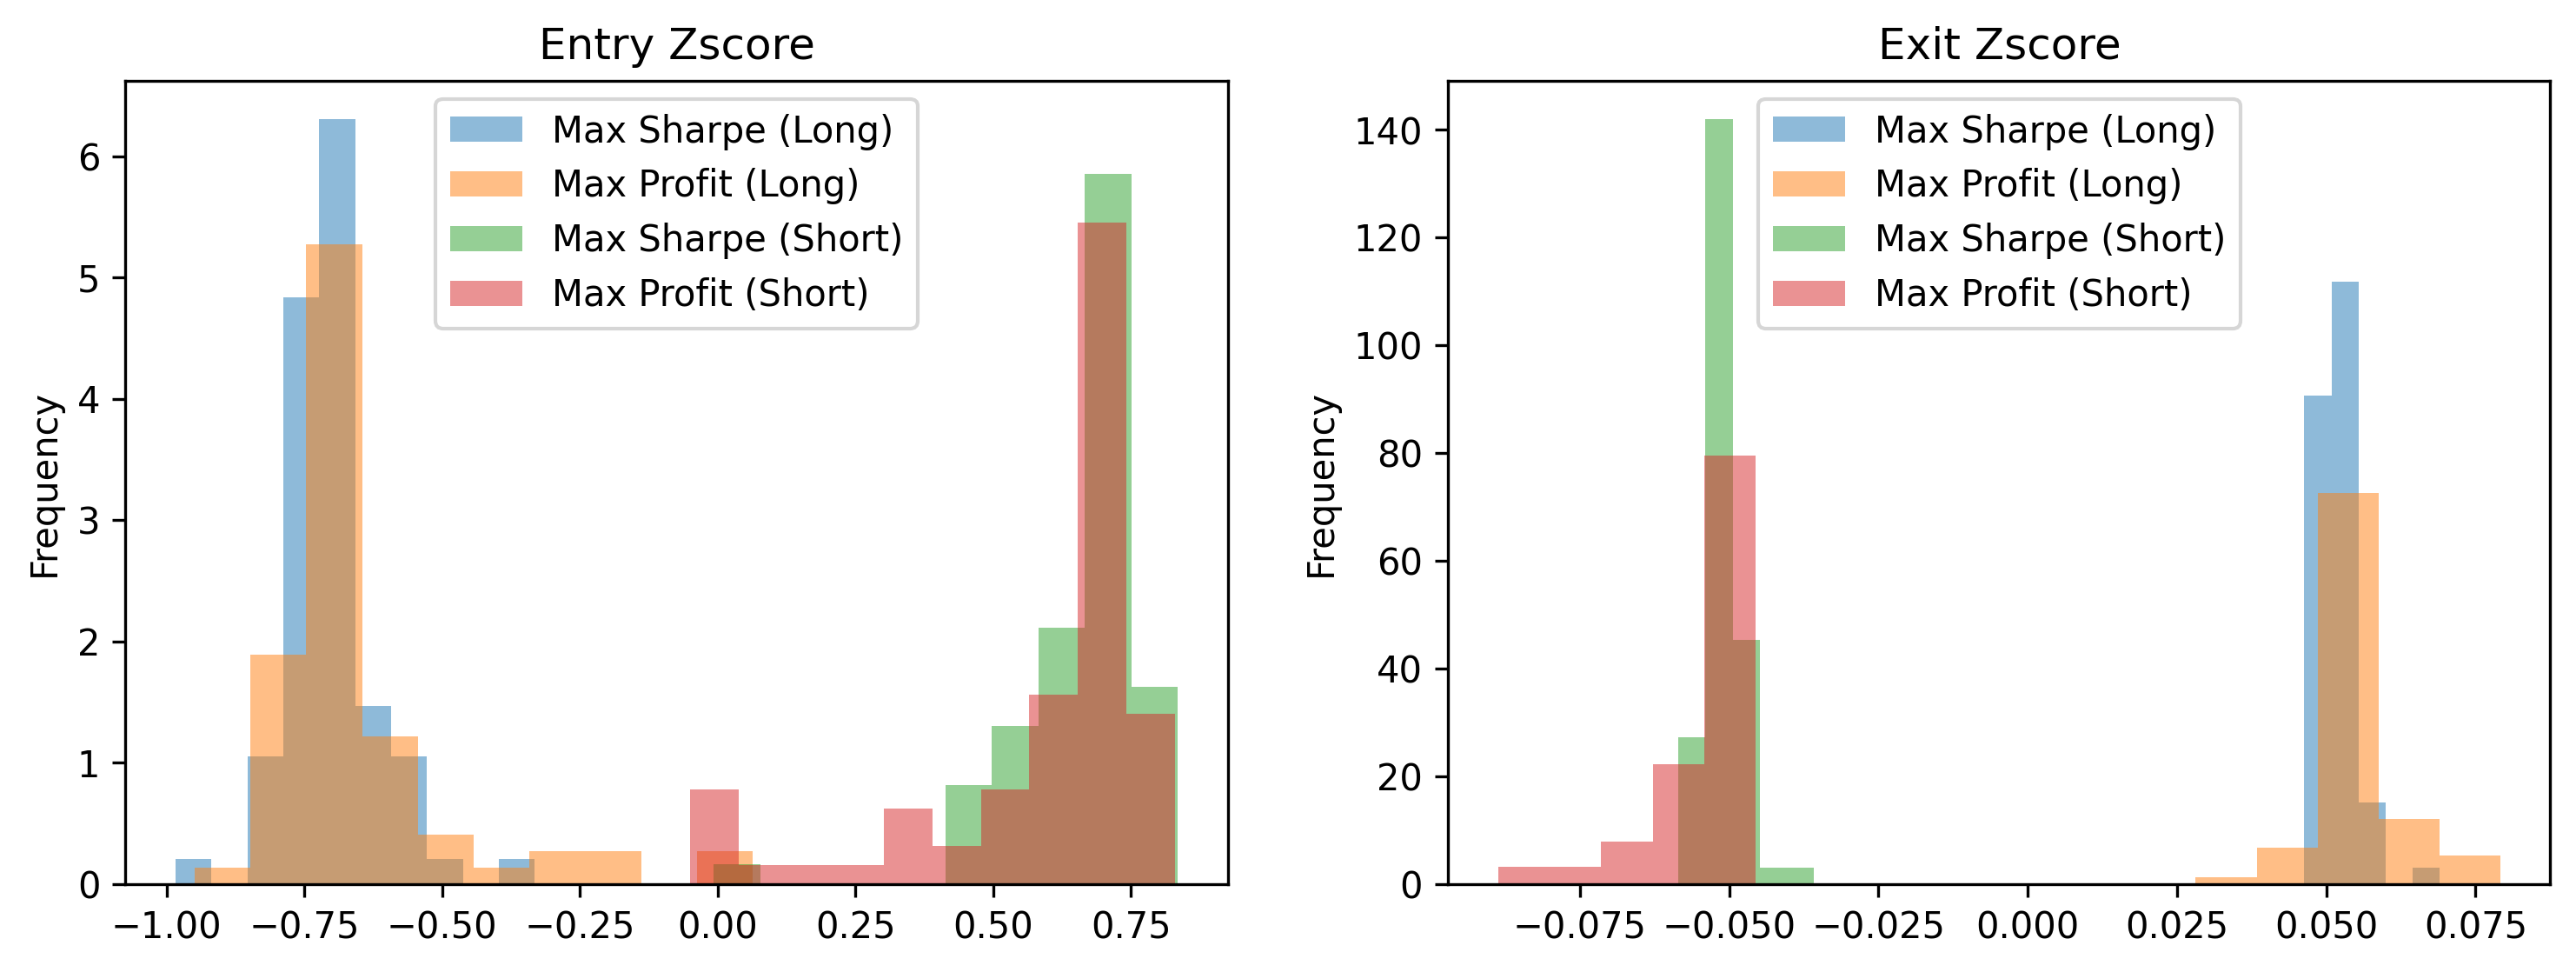
\includegraphics[width=0.78\textwidth]{zscore_optim.png}
\caption{Distribution of the optimized entry and exit thresholds.}
\label{fig:zoptim}
\end{figure}

\begin{figure}[thbp]
\centering
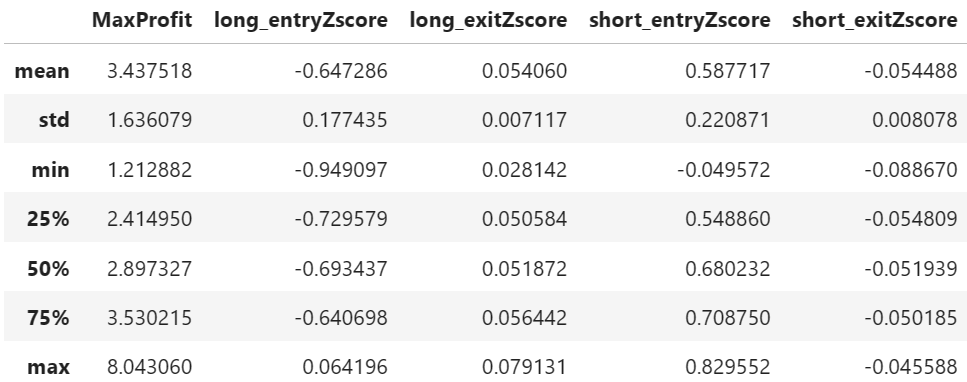
\includegraphics[width=0.45\textwidth]{MaxProfit_describe.png}
\hfill
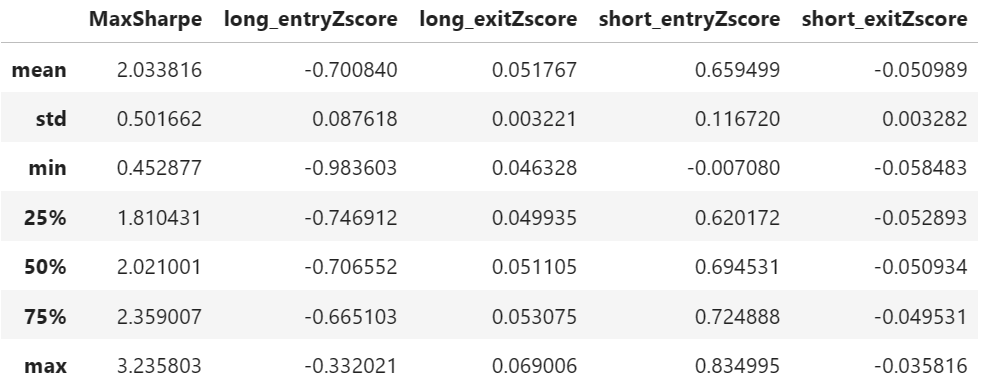
\includegraphics[width=0.45\textwidth]{MaxSharpe_describe.png}
\caption{Summary statistics of the optimized thresholds under the maximum profit (LHS) and maximum Sharpe ratio (RHS) objective.}
\label{fig:zdesc}
\end{figure}

\section{Portfolio Weighting}

\subsection{Confidence Score}

Since equal weighting ignores the fact that the 73 pairs differ in how reliably they revert, we propose a confidence score based on the rolling cointegration statistics and forecast volatility. The first is the strength of the cointegration relationship over a trailing window of $r = 250$ trading days, measured either by the absolute test statistic $\mathrm{Coint}_t(i,r)$ or by the p-value $\mathrm{Coint}_p(i,r)$. The second is the forecast volatility of the spread, on the reasoning that when a position is opened at an extreme z-score, a more volatile spread is more likely to return toward its mean than to move further away. 
\begin{equation}
\gamma_t(i) = h_i \cdot \mathrm{Coint}_t(i, r), \qquad \gamma_p(i) = \frac{h_i}{\mathrm{Coint}_p(i, r)},
\end{equation}
with $h_i$ the forecast volatility of spread $i$. Both are recomputed at every date, so the allocation responds to a pair whose cointegration weakens during the testing period.

\subsection{Weight Calculation}

While we should allocate more weight to confident pairs, we want to prevent any single pair from dominating the book. Therefore, we cap it at four times the equally weighted share, $c = \frac{4}{n}$, about 5.5\% at $n = 73$. Let $A_k$ be the set of pairs assigned a weight after $k$ passes, starting with $A_0 = \emptyset$, and let $R_k = 1 - \sum_{i \in A_k} w_i$ be the remaining unassigned weight. Pass $k+1$ assigns
\begin{equation}
w_i = R_k\, c \qquad \text{for every } i \notin A_k \text{ with } \frac{\gamma_i}{\sum_{j \notin A_k} \gamma_j} > R_k\, c, \text{ subject to }
\sum_{i=1}^{n} w_i = 1 .
\label{eq:cap}
\end{equation}
and the passes repeat until no further pair qualifies. Since $R_k$ falls at every pass, the effective cap tightens as capital is committed. Pairs never assigned receive the smallest assigned weight, and the vector is rescaled to satisfy the constraint.

\section{Backtest Results}

Three strategies are compared. \EWFE{} weights the pairs equally and uses one fixed threshold pair for all of them, entering at $\pm 0.8$ and exiting at $\mp 0.05$. \EWOE{} weights the pairs equally and uses optimized thresholds. \OWOE{} uses the confidence weight and optimized thresholds. All three run through the same BackTrader \texttt{Cerebro} engine with one data feed per underlying. Signals are read from the output of the previous sections, orders are submitted at market and fill at the opening price of the following bar, transaction cost is 0.1\% of traded notional on each side and no slippage is applied. The evaluation window is the 593 trading days from 23 August 2021 to 29 December 2023.

\begin{table}[thbp]
\centering
\begin{tabular}{lccc}
\toprule
 & \EWFE{} & \EWOE{} & \OWOE{} \\
\midrule
Total return           & 158.68\% & 179.99\% & 202.22\% \\
Sharpe ratio           & 1.32     & 1.17     & 1.43     \\
Maximum drawdown       & 28.58\%  & 32.75\%  & 25.59\%  \\
System quality number  & 3.68     & 2.72     & 3.28     \\
Number of trades       & 540      & 386      & 393      \\
\bottomrule
\end{tabular}
\caption{Strategy metrics over the evaluation window, net of transaction costs.}
\label{tab:metrics}
\end{table}

Table \ref{tab:metrics} reports performance over the window. Optimizing the thresholds does not pay for itself. \EWFE{} has an annualized volatility of 33.7\% and a drawdown of 28.58\%, compared to \EWOE{}'s 44.2\% and its drawdown of 32.75\%. Despite a higher return, the Sharpe ratio of 1.17 is lower than 1.32. Nevertheless, the confidence weighting, together with optimized thresholds, delivers the best performance. \OWOE{} earns the highest return, but the volatility of 36.2\% and 25.59\% drawdown are much lower. The Sharpe ratio is the highest at 1.43, while the number of trades is almost unchanged at 393 against 386 for \EWOE{}. Focusing on pairs with strong cointegration and volatile spreads improves both risk and return. Figures \ref{fig:bt} and \ref{fig:btow} show the portfolio value, cash, per-trade profit and loss and drawdown paths behind these results.

\begin{figure}[thbp]
\centering
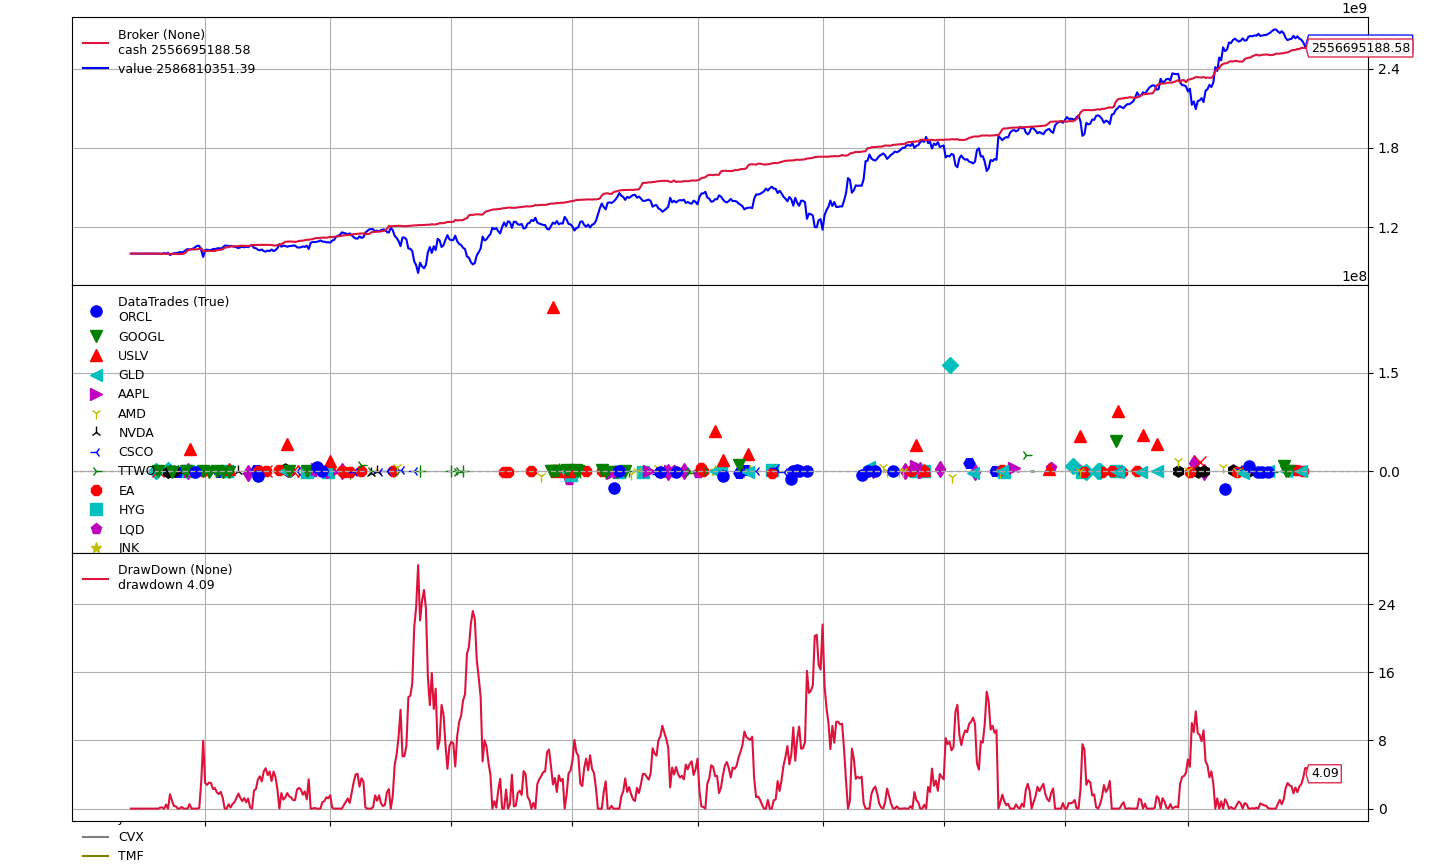
\includegraphics[width=\linewidth]{EW-FE.png}
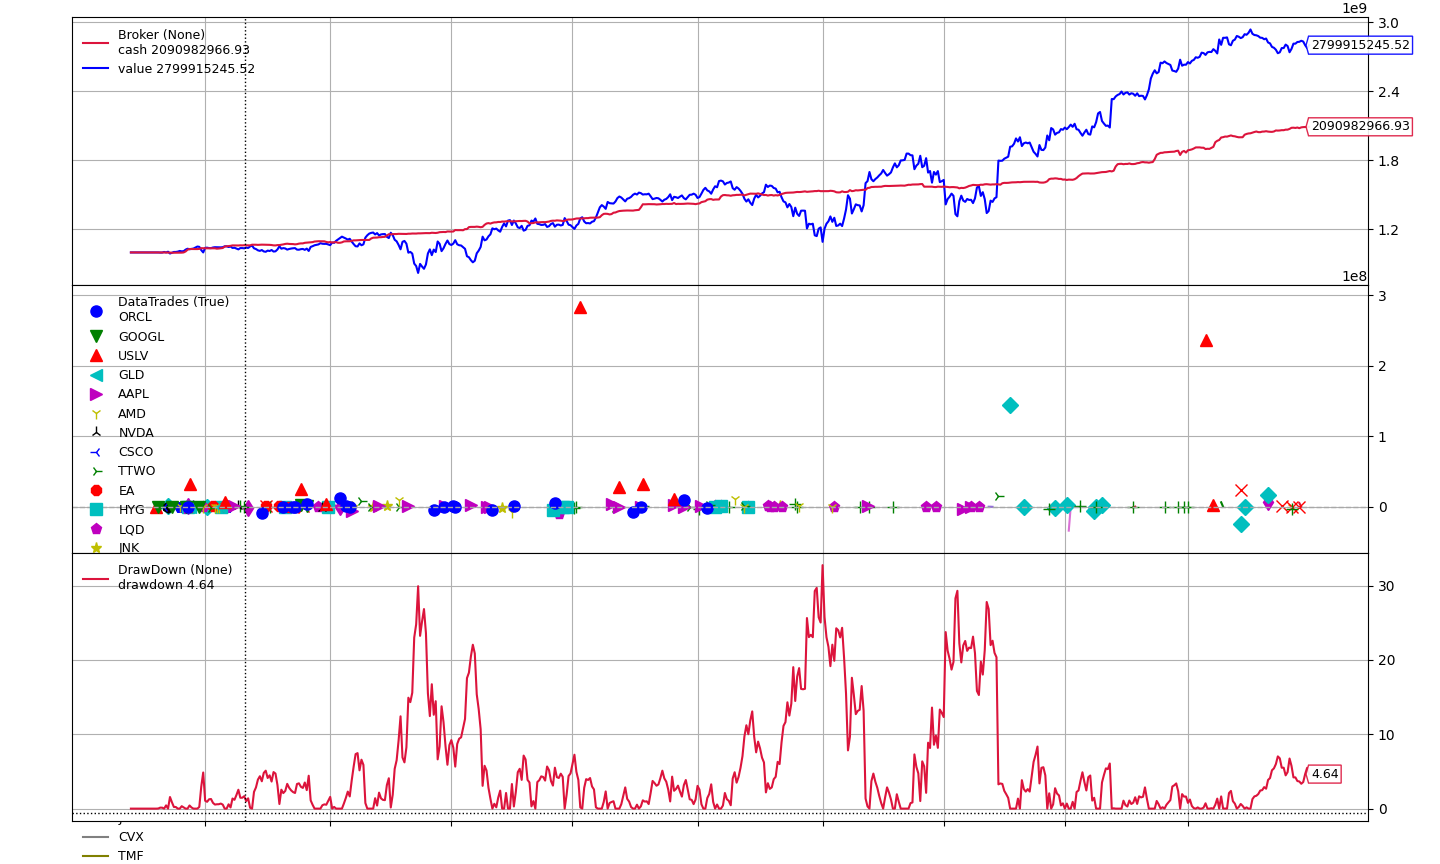
\includegraphics[width=\linewidth]{EW-OE.png}
\caption{Backtest paths for \EWFE{}, upper, and \EWOE{}, lower. Each panel reports portfolio value, cash, per-trade profit and loss and drawdown.}
\label{fig:bt}
\end{figure}

\begin{figure}[thbp]
\centering
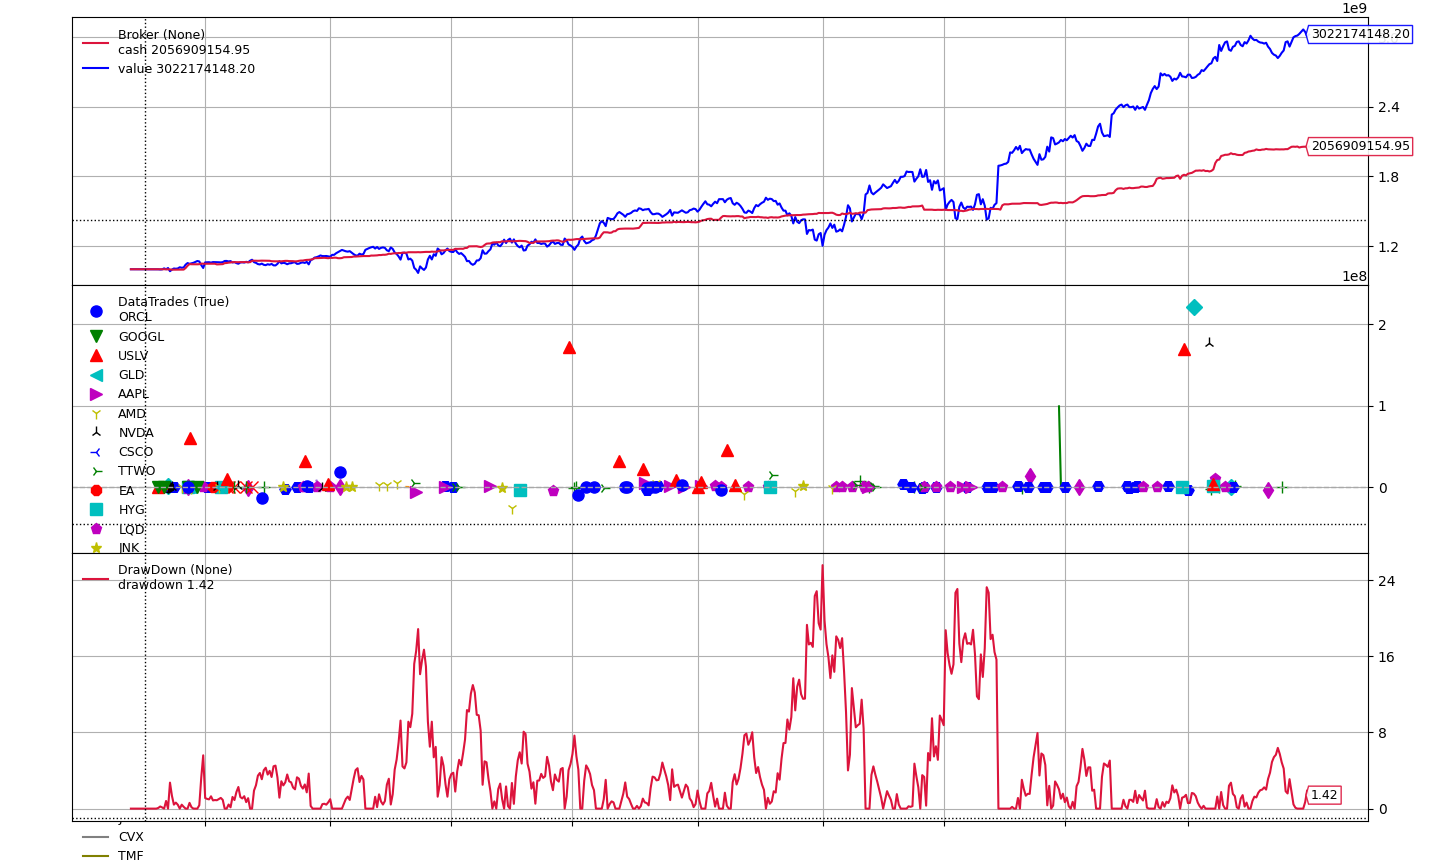
\includegraphics[width=\linewidth]{OW-OE.png}
\caption{Backtest paths for \OWOE{}.}
\label{fig:btow}
\end{figure}

\section{Conclusion}

In this project, we optimize the entry and exit thresholds and propose a confidence-weighting scheme. Optimizing the thresholds pair by pair improves returns but increases volatility and drawdown by more, so the risk-adjusted measure decreases. Combined with a confidence score based on the rolling cointegration statistic and forecast volatility, it delivers the highest total return, the highest Sharpe ratio and the lowest drawdown.

\newpage
\begin{thebibliography}{99}
\bibitem[Engle(1982)]{engle1982} Engle, R. F. (1982). Autoregressive conditional heteroscedasticity with estimates of the variance of United Kingdom inflation. \textit{Econometrica}, 50(4), 987--1007.
\bibitem[Engle(2002)]{engle2002} Engle, R. F. (2002). Dynamic conditional correlation. \textit{Journal of Business and Economic Statistics}, 20(3), 339--350.
\bibitem[Engle and Granger(1987)]{engle1987} Engle, R. F. and Granger, C. W. J. (1987). Co-integration and error correction. \textit{Econometrica}, 55(2), 251--276.
\bibitem[Jarque and Bera(1980)]{jarque1980} Jarque, C. M. and Bera, A. K. (1980). Efficient tests for normality, homoscedasticity and serial independence of regression residuals. \textit{Economics Letters}, 6(3), 255--259.
\bibitem[Kalman(1960)]{kalman1960} Kalman, R. E. (1960). A new approach to linear filtering and prediction problems. \textit{Journal of Basic Engineering}, 82(1), 35--45.
\bibitem[Nelson(1991)]{nelson1991} Nelson, D. B. (1991). Conditional heteroskedasticity in asset returns. \textit{Econometrica}, 59(2), 347--370.
\bibitem[Shapiro and Wilk(1965)]{shapiro1965} Shapiro, S. S. and Wilk, M. B. (1965). An analysis of variance test for normality. \textit{Biometrika}, 52(3), 591--611.
\end{thebibliography}

\newpage
\appendix

\section{Supplementary Figures}
\begin{figure}[thbp]
\centering
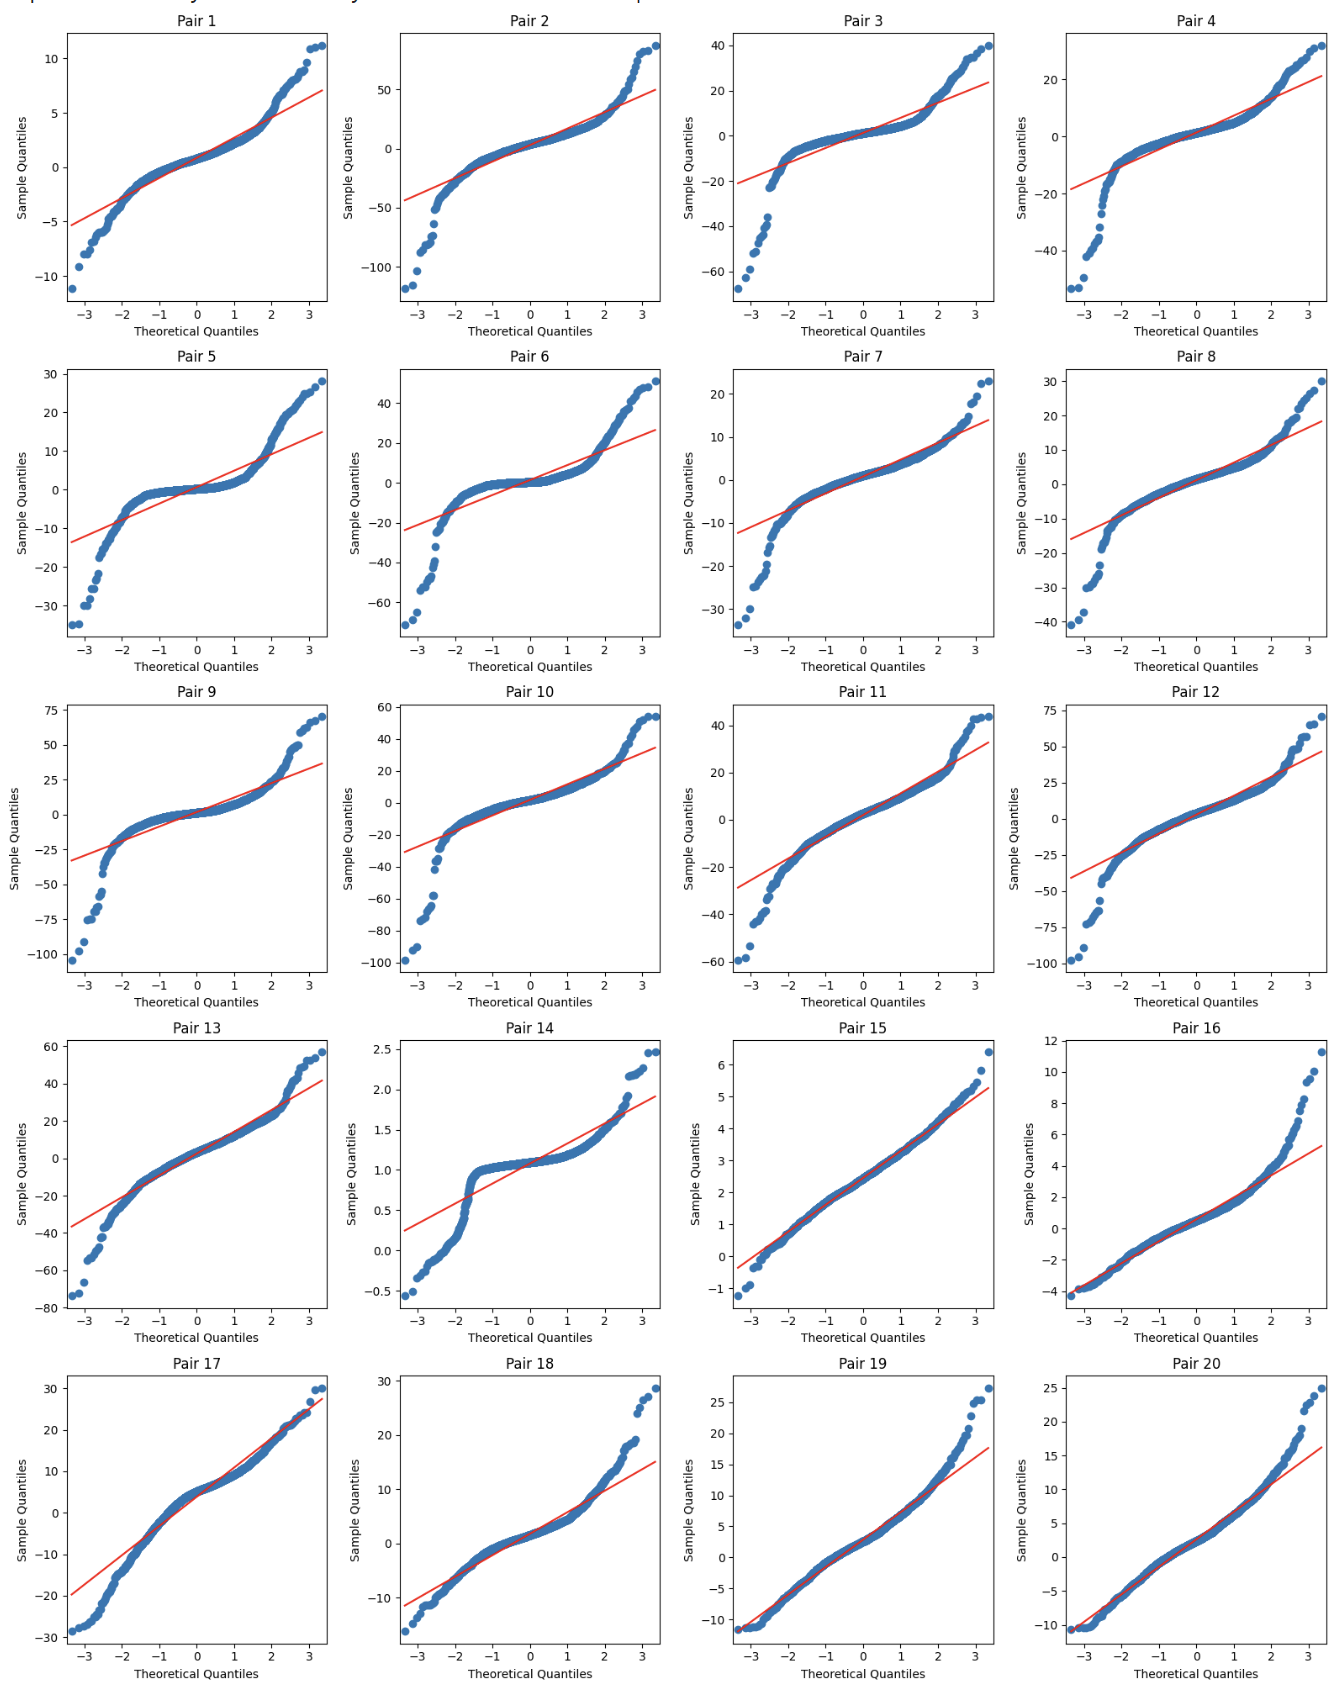
\includegraphics[width=0.32\textwidth]{QQ_plot_1.png}
\hfill
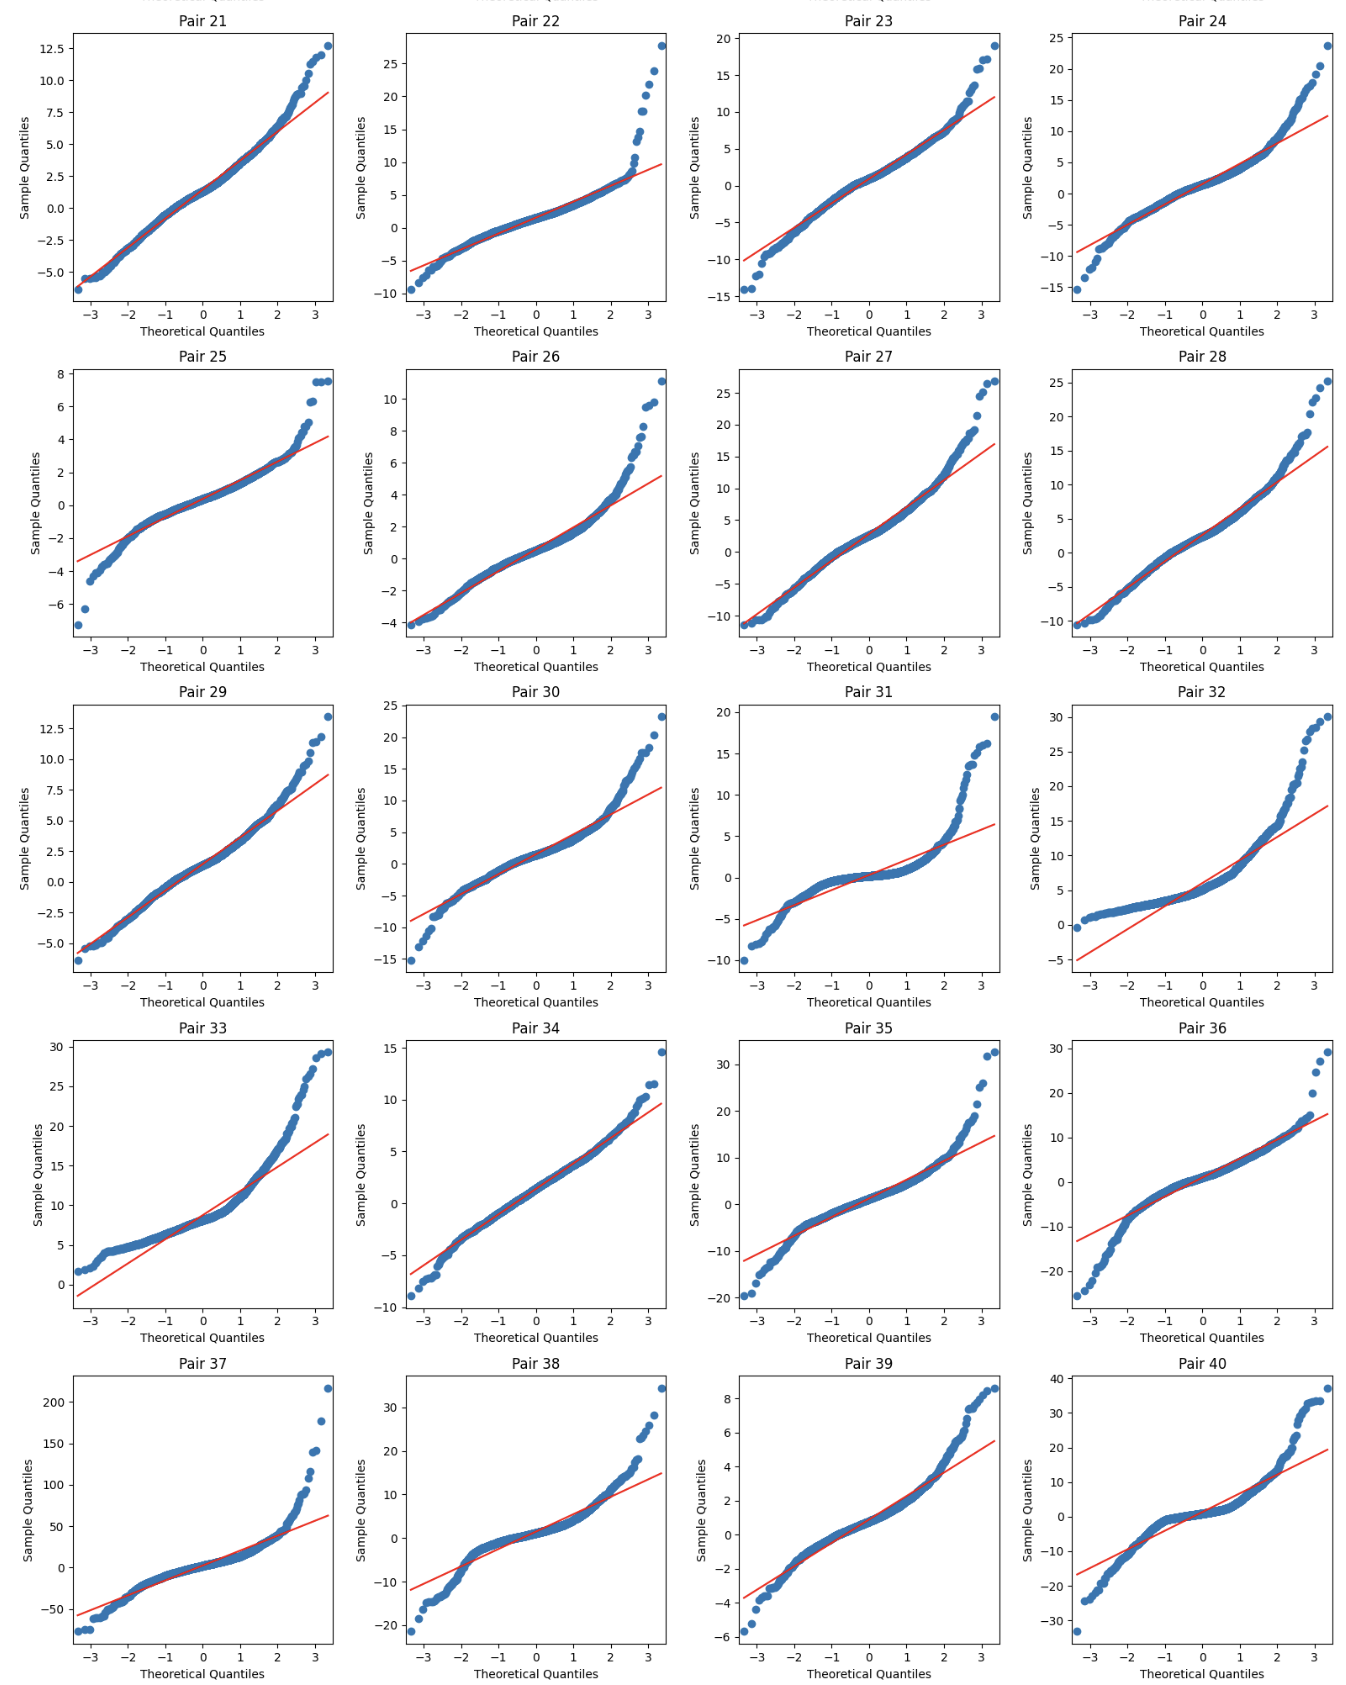
\includegraphics[width=0.32\textwidth]{QQ_plot_2.png}
\hfill
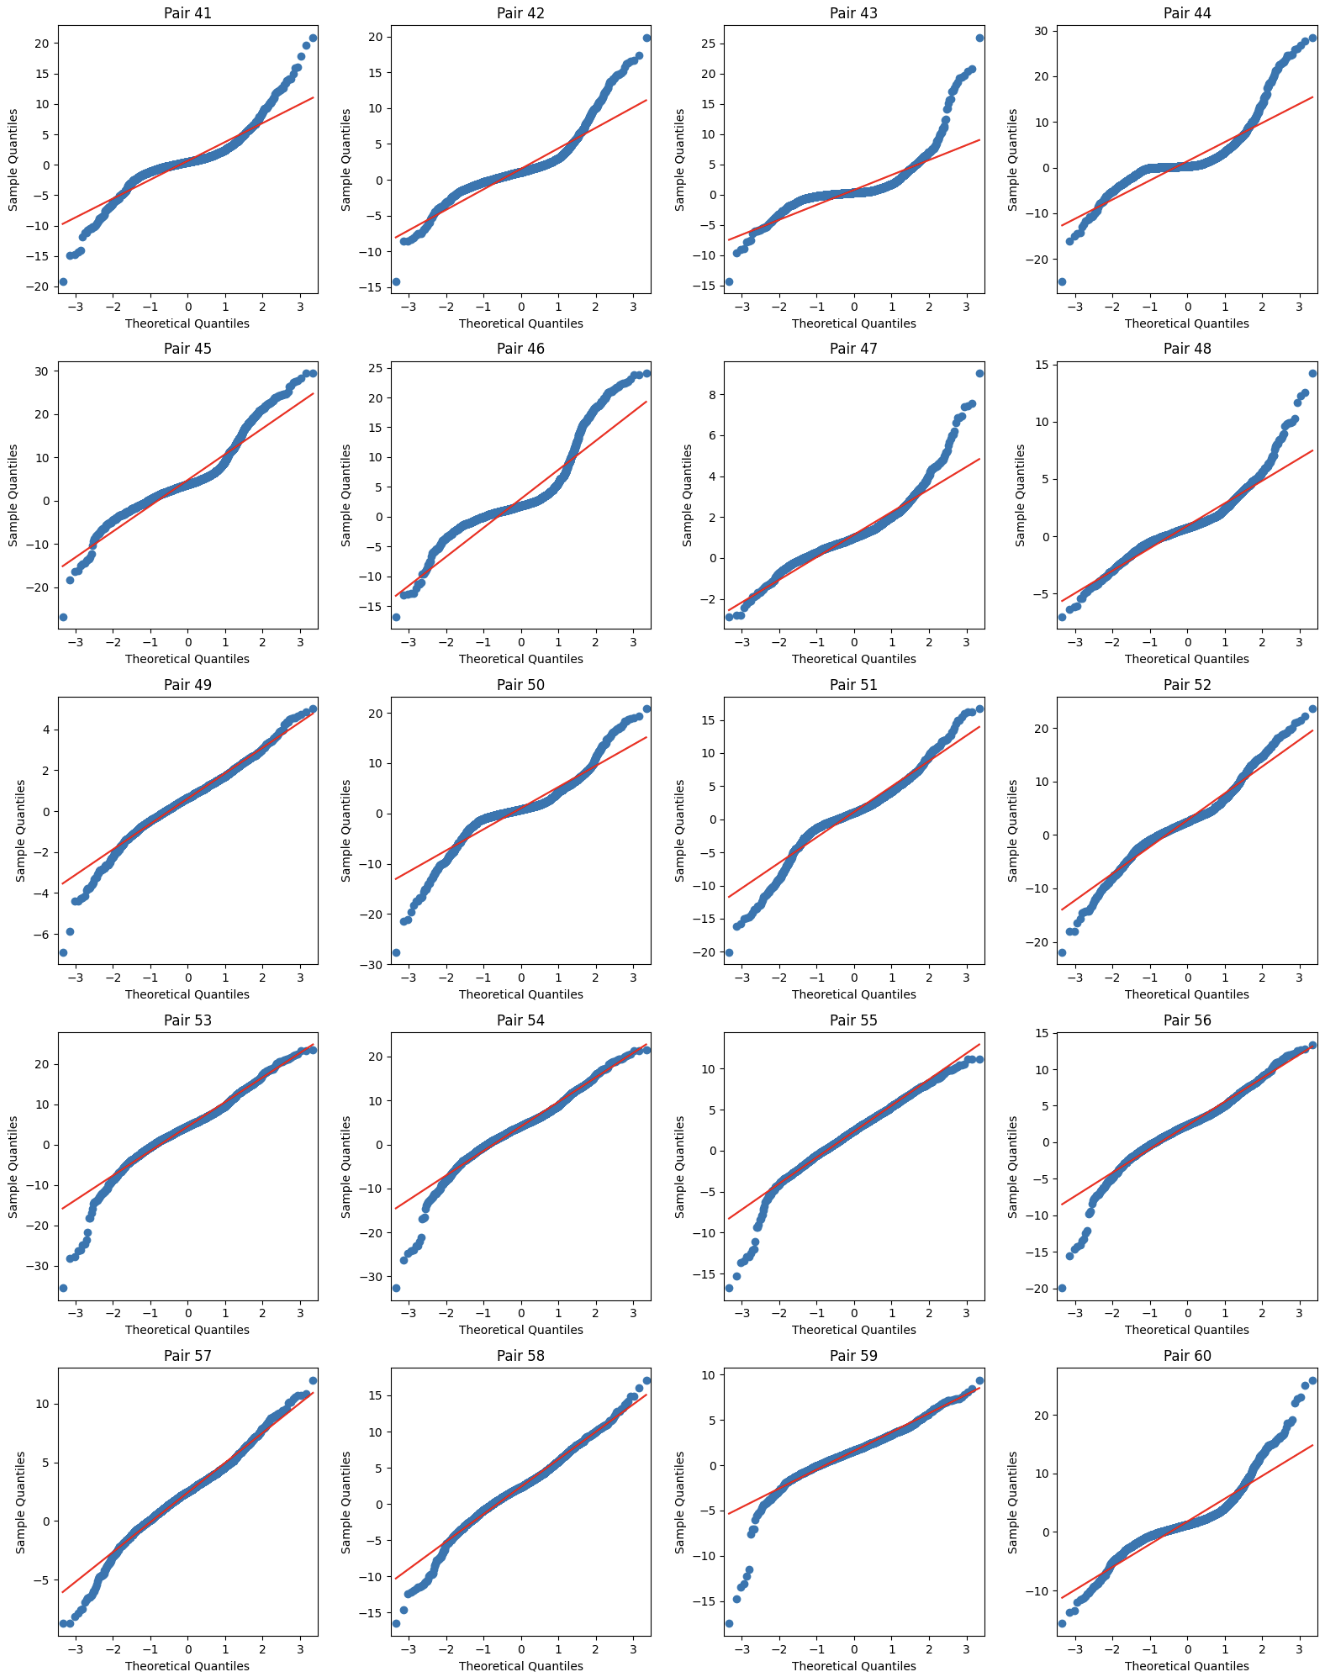
\includegraphics[width=0.32\textwidth]{QQ_plot_3.png}
\caption{Quantile-quantile plots of training spreads against the Gaussian.}
\label{fig:qq}
\end{figure}

\end{document}
